%*****************************************
\chapter{Forecasting}\label{ch08:forecasting}
%*****************************************

One of the most powerful features of Excel is the ability to analyze data and create charts with trend lines that would help business people forecast future conditions. It also contains several tools designed for ``what-if'' analysis where business people can project the results of changing market variables or corporate decisions. This chapter introduces all of these features. 

\section{Advanced Charts}

\begin{center}
	\begin{objbox}{Learning Objectives}
		\begin{itemize}
			\setlength{\itemsep}{0pt}
			\setlength{\parskip}{0pt}
			\setlength{\parsep}{0pt}
			
			\item Sparklines graphically represent data trends in a single cell.
			\item Trendlines simplify graphs to display a single trend line.
			\item Forecast Worksheets create a trendline but include confidence levels.
			\item Filled maps are depictions of geographically-related data like the locations of a company's customers.

		\end{itemize}
	\end{objbox}
\end{center}

\subsection{Sparklines}

Sparklines are tiny graphs that visually represent data in a single worksheet cell. These are powerful ways to help managers quickly ``see'' the data.

\begin{enumerate}
	\item Open workbook \fmtWorkbookName{CH8-Sparkline.xlsx}
	\item Open the \fmtWorksheetName{Precipitation} worksheet.
\end{enumerate}

This worksheet contains the average monthly precipitation for ten United States cities (data from  \url{https://www.usclimatedata.com/climate/united-states/us}).

\begin{enumerate}[resume]
	\item Click cell \fmtCellLocation{N4} to activate that location.
	\item Click \fmtRibbonButton{Insert $ \Rightarrow $ Sparklines $ \Rightarrow $ Line}.
\end{enumerate}

\begin{figure}[H]
	\centering
	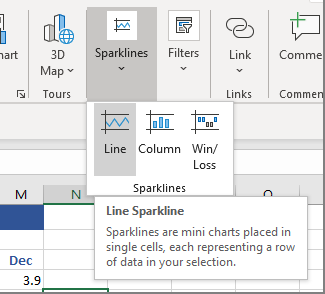
\includegraphics[width=\maxwidth{.95\linewidth}]{gfx/ch08_fig01}
	\caption{The Sparklines Button}
	\label{08:fig01}
\end{figure}

\begin{enumerate}[resume]
		
	\item For the Data Range, enter \fmtTyping{B4:M4}.
	\item For the Location Range, enter \fmtTyping{\$N\$4}.
	\item Click \fmtPopupButton{OK}.
\end{enumerate}

\begin{figure}[H]
	\centering
	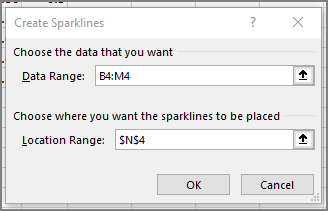
\includegraphics[width=\maxwidth{.95\linewidth}]{gfx/ch08_fig02}
	\caption{The Sparklines Diaglog Box}
	\label{08:fig02}
\end{figure}

Excel creates a tiny line graph that shows the monthly precipitation for the entire year. 

\begin{figure}[H]
	\centering
	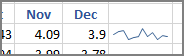
\includegraphics[width=\maxwidth{.95\linewidth}]{gfx/ch08_fig03}
	\caption{One Sparkline}
	\label{08:fig03}
\end{figure}

\begin{enumerate}[resume]
	\item Copy/paste cell \fmtCellLocation{N4} to \fmtCellLocation{N5:N13}. The fill handle will make this easier. 
\end{enumerate}

\begin{figure}[H]
	\centering
	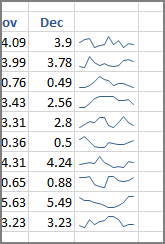
\includegraphics[width=\maxwidth{.95\linewidth}]{gfx/ch08_fig04}
	\caption{All Sparklines In Place}
	\label{08:fig04}
\end{figure}

Now Excel displays a sparkline for each of the cities. While it is not possible to see the details for any specific month and city, it is easy to spot trends. For example, Portland OR has less precipitation in the late summer while Chicago IL seems to start out slow in January and then grow through the spring and early summer. A business manager could use a sparkline to easily detect trends in data.

\begin{enumerate}[resume]
	\item Select \fmtCellLocation{N4:N13}.
	\item Click \fmtRibbonButton{Sparkline $ \Rightarrow $ Type $ \Rightarrow $ Column}.
\end{enumerate}

\begin{figure}[H]
	\centering
	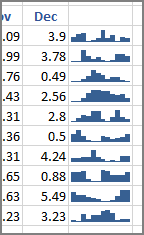
\includegraphics[width=\maxwidth{.95\linewidth}]{gfx/ch08_fig05}
	\caption{Column Sparklines}
	\label{08:fig05}
\end{figure}

The sparklines change into column graphs. The information does not change, but it may be easier to spot trends with one type of graph or the other, so it is a best practice to try both.

\begin{enumerate}[resume]
	\item Open the \fmtWorksheetName{Temperature} worksheet in the \fmtWorkbookName{CH8-Sparkline} workbook.
\end{enumerate}

This worksheet contains the average low temperature for five Alaskan cities (data from  \url{https://www.usclimatedata.com/climate/united-states/us}).

\begin{enumerate}[resume]
	\item Click cell \fmtCellLocation{N4} to activate that location.
	\item Click \fmtRibbonButton{Insert $ \Rightarrow $ Sparklines $ \Rightarrow $ Win/Loss}.
	\item For the Data Range, enter \fmtTyping{B4:M4}.
	\item For the Location Range, enter \fmtTyping{\$N\$4}.
	\item Click \fmtPopupButton{OK}.
	\item Click \fmtCellLocation{N4} and notice the \fmtRibbonTab{Sparkline} tab includes several options to modify the appearance of the sparkline. 
	\item Copy \fmtCellLocation{N4} to \fmtCellLocation{N5:N8}, the fill handle will make this easier.
\end{enumerate}

\begin{figure}[H]
	\centering
	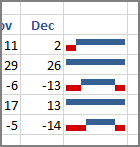
\includegraphics[width=\maxwidth{.95\linewidth}]{gfx/ch08_fig06}
	\caption{Win/Loss Sparkline}
	\label{08:fig06}
\end{figure}

Excel creates a bar graph that shows positive values in blue and negative values in red. This does not show the magnitude of each value, but only whether it is positive or negative in nature. This type of sparkline is useful for quickly determining things like if a stock price is increasing or decreasing.

\subsection{Trend Lines}

Excel can easily create trend lines on graphs to indicate the data trends. These lines can be extended to forecast how the data may move in the near future.

\begin{enumerate}
	\item Open workbook \fmtWorkbookName{CH8-Dow}.
\end{enumerate}

This workbook contains the closing Dow Jones average for each month from $ 1981 $–$ 1990 $.

\begin{enumerate}[resume]
	\item Click cell \fmtCellLocation{A1} to activate that location.
	\item Click \fmtRibbonButton{Insert $ \Rightarrow $ Charts $ \Rightarrow $ Recommended Charts}.
	\item Select the line chart (it is the second selection).
	\item Click \fmtPopupButton{OK}.
	\item Click in the chart area and then click the $ + $ button at the top right corner of the chart to add chart elements.

\end{enumerate}

\begin{figure}[H]
	\centering
	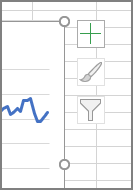
\includegraphics[width=\maxwidth{.95\linewidth}]{gfx/ch08_fig07}
	\caption{Adding Chart Elements}
	\label{08:fig07}
\end{figure}

\begin{enumerate}[resume]

	\item Hover the mouse over the \fmtPopupButton{Trendline} button, then click the arrow beside the button.

\end{enumerate}

\begin{figure}[H]
	\centering
	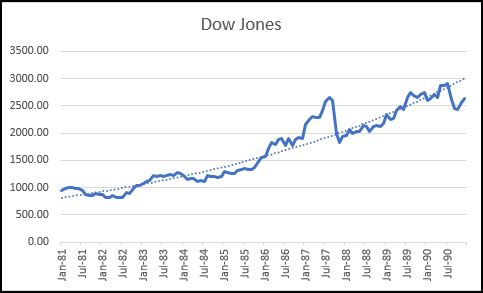
\includegraphics[width=\maxwidth{.95\linewidth}]{gfx/ch08_fig08}
	\caption{The Trendline Button}
	\label{08:fig08}
\end{figure}

\begin{enumerate}[resume]
	
	\item Select \fmtPopupButton{More Options} from the \fmtPopupBox{Trendline} popup menu.
	\item Click the \fmtPopupButton{Exponential} radio button to select that option. \textit{Note}: it is reasonable to click on each of the types of trend lines to see which seems to best fit the data.
\end{enumerate}

\begin{figure}[H]
	\centering
	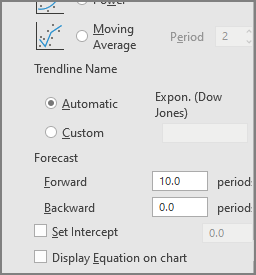
\includegraphics[width=\maxwidth{.95\linewidth}]{gfx/ch08_fig09}
	\caption{Trendline Added to Graph}
	\label{08:fig09}
\end{figure}

Excel draws a dotted trendline that shows the growth of the Dow over the ten-year period.

\begin{enumerate}[resume]
	\item Enter \fmtTyping{10} for the \fmtPopupBox{Forward Forcast} period to extend the trendline out five years (ten six-month periods).
\end{enumerate}

\begin{figure}[H]
	\centering
	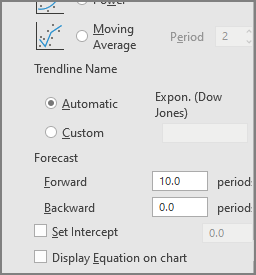
\includegraphics[width=\maxwidth{.95\linewidth}]{gfx/ch08_fig10}
	\caption{Extending The Trendline for 10 Periods}
	\label{08:fig10}
\end{figure}

Excel forecasts a generally upward trend for the five-year period.

\begin{figure}[H]
	\centering
	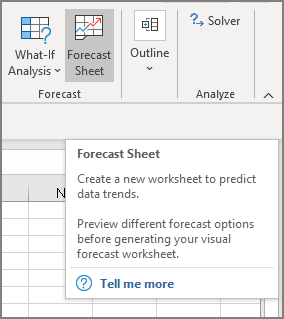
\includegraphics[width=\maxwidth{.95\linewidth}]{gfx/ch08_fig11}
	\caption{Trendline With Forecast}
	\label{08:fig11}
\end{figure}

\subsection{Forecast Worksheet}

The trend lines described above are easy to add to a chart, but Excel includes a tool called Forecast Worksheet that creates a forecast along with confidence levels.

\begin{enumerate}
	\item Open workbook \fmtWorkbookName{CH8-Dow} if it is not already open.
\end{enumerate}

This workbook contains the closing Dow Jones average for each month from $ 1981 $–$ 1990 $.

\begin{enumerate}[resume]
	\item Click cell \fmtCellLocation{A1} to activate that location.
	\item Click \fmtRibbonButton{Data $ \Rightarrow $ Forecasts $ \Rightarrow $ Forecast Sheet}.
\end{enumerate}

\begin{figure}[H]
	\centering
	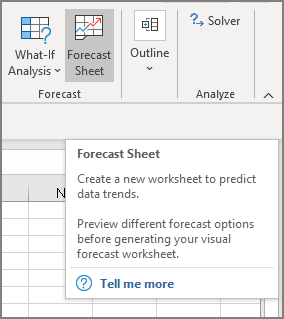
\includegraphics[width=\maxwidth{.95\linewidth}]{gfx/ch08_fig12}
	\caption{The Forecast Sheet Button}
	\label{08:fig12}
\end{figure}

\begin{enumerate}[resume]
	
	\item The default options are appropriate for this exercise. Here are what the other options do.
	
	\begin{itemize}
		\item Forecast End. Set an end date for the forecast, which are the orange lines in the illustration.
		\item Forecast Start. Set the start dae for the forecast.
		\item Confidence interval. This is a statistical value that indicates a $ 95 $\% certainty that as time progresses the graph will fall between the upper and lower limits shown. The confidence interval can be adjusted, but $ 95 $\% is common.
		\item Seasonality. Excel will search for any sort of seasonal cycles and adjust the forecast accordingly.
		\item Timeline and Values Range. This is the data that was used to create the graph. If Excel got the wrong data ranges then they can be adjusted here.
		\item Fill Missing Points Using. This tells Excel how to deal with data points that are missing. It will either fill those missing values with zero or interpolate a value between the two neighboring values. Interpolation is usually the best option.
		\item Aggregate Duplicates Using. There are a number of options available for aggregating duplicates in the data. Average is usually the best option.
	\end{itemize}	
	
	\item Click \fmtPopupButton{Create}.

\end{enumerate}

\begin{figure}[H]
	\centering
	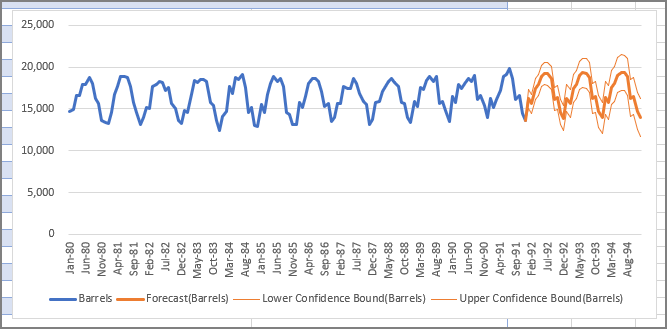
\includegraphics[width=\maxwidth{.95\linewidth}]{gfx/ch08_fig13}
	\caption{Dow Forecast}
	\label{08:fig13}
\end{figure}

\begin{enumerate}[resume]
	\item Excel creates a new worksheet containing the chart along with a table listing all of the values used to create the chart.
	\item As a second example, open workbook \fmtWorkbookName{CH8-Beer}. This workbook contains the total United States beer production, in barrels, for January, 1980, until December, 1991. 
	\item Click in \fmtCellLocation{A1} to select that location.
	\item Click \fmtRibbonButton{Data $ \Rightarrow $ Forecast $ \Rightarrow $ Forecast Sheet}.
	\item Accept the default options and click \fmtPopupButton{Create}.
	\item The graph clearly shows the cyclic nature of beer production and forecasts a similar cycle out to December, 1994.
\end{enumerate}

\begin{figure}[H]
	\centering
	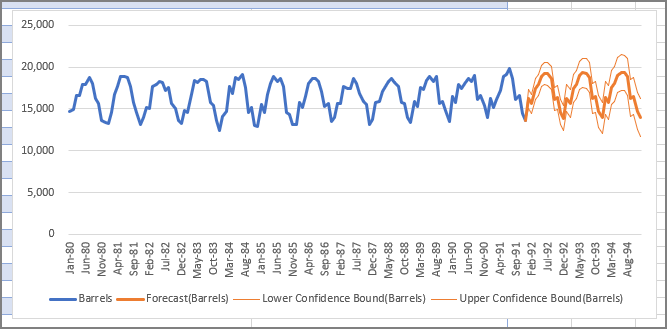
\includegraphics[width=\maxwidth{.95\linewidth}]{gfx/ch08_fig14}
	\caption{Beer Production Forecast}
	\label{08:fig14}
\end{figure}

A forecast sheet is a simple method to predict business cycles like customer demand so owners can manage inventory, hire help, or take other actions.

\subsection{Filled Map}

Excel is able to create a map if data includes any sort of geographical identifiers, like country names, states, counties, or cities. 

\begin{enumerate}
	\item Open workbook \fmtWorkbookName{CH8-CancerRate}.
\end{enumerate}

This workbook contains the rate of cigarette smoking along with cancer rates for various types of cancer that seem to be related to smoking. The data was captured in a study completed in $ 1960 $.

\begin{enumerate}[resume]
	\item Click cell \fmtCellLocation{A3:B43} to activate that range of cells.
	\item Click \fmtRibbonButton{Insert $ \Rightarrow $ Charts $ \Rightarrow $ Maps}.
	\item Select \fmtRibbonButton{Filled Map}.
	\item Click the map icon.
\end{enumerate}

\begin{figure}[H]
	\centering
	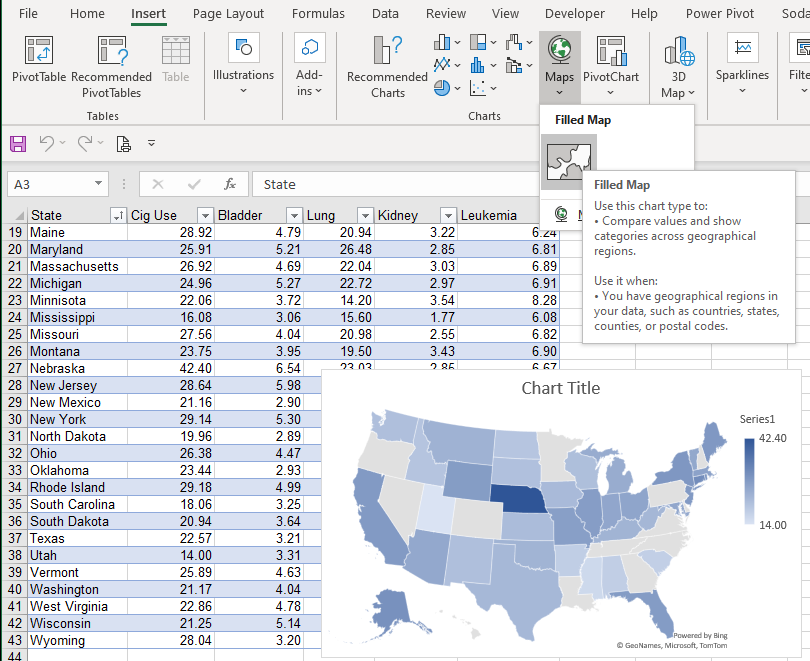
\includegraphics[width=\maxwidth{.95\linewidth}]{gfx/ch08_fig15}
	\caption{Creating a Filled Map}
	\label{08:fig15}
\end{figure}

\begin{enumerate}[resume]	
	\item Excel creates a map of the United States with the cigarette use rate indicated by color. Nebraska has the highest rate of cigarette use and states that are gray, like Oregon, did not have data in the input table.
	\item Click the chart title two times to enable editing. Change that title to \fmtTyping{Cigarette Use}.
	\item Click the paint brush tool at the top right corner of the map to change the style and colors for the map. Click \fmtPopupButton{Color} in the popup menu.
	\item Select \fmtPopupButton{Monochromatic Palette 6}, a green palette.
\end{enumerate}

\begin{figure}[H]
	\centering
	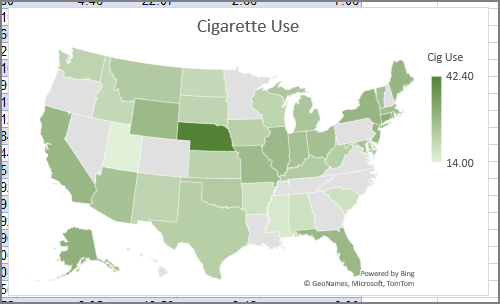
\includegraphics[width=\maxwidth{.95\linewidth}]{gfx/ch08_fig16}
	\caption{Completed Map}
	\label{08:fig16}
\end{figure}

In the same way that the cigarette use rate was mapped, any of the types of cancer can be mapped. The limitation is that only one variable, plus the state names, can be mapped at one time. However, this is a great way for managers to determine, for example, where their customers live so they can plan some sort of promotion.

\begin{center}
	\begin{tkwbox}{Key Take-Aways}
		\textbf{Advanced Charts}
		\\
		\begin{itemize}
			\setlength{\itemsep}{0pt}
			\setlength{\parskip}{0pt}
			\setlength{\parsep}{0pt}
			
			\item Sparklines graphically represent data trends in a single cell. These are quick and easy to add to a worksheet and provide managers readily available important information.
			\item Trend lines simplify graphs by displaying a single trend line to summarize the general direction of the data. There are several different trend lines available in Excel and those lines can be modified to enhance their appearance.
			\item Forecast Worksheets create a trend line that includes confidence levels. These worksheets are also more robust than simple trend lines and can analyze cyclic or seasonal data.
			\item Filled maps present geographically-related data in a map. These are automatically created so the designer does not need to know anything about map-making. These are useful to plot customer locations in order to better focus marketing campaigns.
			
		\end{itemize}
	\end{tkwbox}
\end{center}

\section{What-If Analysis}

\begin{center}
	\begin{objbox}{Learning Objectives}
		\begin{itemize}
			\setlength{\itemsep}{0pt}
			\setlength{\parskip}{0pt}
			\setlength{\parsep}{0pt}
			
			\item Data tables permit numeric analysis of the result of changing inputs.
			\item Scenarios create various sets of inputs to compare the resulting output.
			\item Goal seeking finds an optimum input to achieve a specific goal.
			\item The Solver performs complex analysis of a scenario and adjusts various parameters for an optimum outcome.
			
		\end{itemize}
	\end{objbox}
\end{center}

\subsection{Data Tables}

Data tables display a range of results for a formula or function as one or two input variables are automatically cycled through a list. Managers can quickly compare potential options to determine a course of action.

\subsubsection{One-Variable Data Table}

As an example of a one-variable data table, imagine that the owner of a small theater wants to predict revenue for the upcoming season. If the revenue from a single ticket sale can be calculated, then that can be put into a formula and revenue projections can be derived.

\begin{enumerate}
	\item Open a new worksheet.
	\item Name the worksheet \fmtWorksheetName{Revenue}.
	\item Enter the following labels.
	
	\begin{itemize}
		\item In cell \fmtCellLocation{A1} enter \fmtTyping{Ticket Sales Last Season}.
		\item In cell \fmtCellLocation{A2} enter \fmtTyping{Revenue Per Ticket}.
		\item In cell \fmtCellLocation{A3} enter \fmtTyping{Revenue Last Season}.
		\item In cell \fmtCellLocation{A4} enter \fmtTyping{Projected Growth}.
		\item In cell \fmtCellLocation{A5} enter \fmtTyping{Revenue this Season}.
	\end{itemize}
	
	\item Adjust the width of column A so the labels fit in the column.
	\item Name cells \fmtCellLocation{B1:B5}. Do this by right-clicking each cell and select \fmtPopupButton{Define Name} from the drop-down menu. Use these names.

	\begin{itemize}
		\item Cell \fmtCellLocation{B1}: \fmtTyping{SalesLastSeason}
		\item Cell \fmtCellLocation{B2}: \fmtTyping{RevenuePerTicket}
		\item Cell \fmtCellLocation{B3}: \fmtTyping{RevenueLastSeason}
		\item Cell \fmtCellLocation{B4}: \fmtTyping{Growth}
		\item Cell \fmtCellLocation{B5}: \fmtTyping{RevenueThisSeason}
	\end{itemize}

	\item Enter these values in column B.

	\begin{itemize}
		\item In cell \fmtCellLocation{B1} enter \fmtTyping{20000}. This is the number of tickets sold last season and will serve as a start point for this season's projection.
		\item In cell \fmtCellLocation{B2} enter \fmtTyping{8}. This is the average revenue, \$$ 8.00 $, that a single ticket generates.
		\item In cell \fmtCellLocation{B3} enter \fmtTyping{=SalesLastSeason * RevenuPerTicket}. This is the total revenue from last season. 
		\item In cell \fmtCellLocation{B4}, enter \fmtTyping{0}. For this analysis, the first assumption is that there is zero growth in ticket sales over last season. This provides a baseline for the other analysis.
		\item In cell \fmtCellLocation{B5}, enter \fmtTyping{=SalesLastSeason * RevenuPerTicket + (Growth * SalesLastSeason)}
	\end{itemize}

\end{enumerate}

\begin{figure}[H]
	\centering
	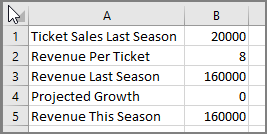
\includegraphics[width=\maxwidth{.95\linewidth}]{gfx/ch08_fig17}
	\caption{The Data Table Parameters}
	\label{08:fig17}
\end{figure}

\begin{enumerate}[resume]
	 
	\item Next, set up the data table area.
	\item In cell \fmtCellLocation{D2}, enter \fmtTyping{Projection}. Bold that cell.
	\item In cell \fmtCellLocation{D3}, enter \fmtTyping{Growth}.
	\item In cell \fmtCellLocation{E3}, enter \fmtTyping{Revenue}.
	\item Leave cell \fmtCellLocation{D4} blank.
	\item In cells \fmtCellLocation{D5:D14}, enter \fmtTyping{0.005}, \fmtTyping{0.01}, \fmtTyping{0.015}, \fmtTyping{0.02}, \fmtTyping{0.025}, \fmtTyping{0.03}, \fmtTyping{0.035}, \fmtTyping{0.04}, \fmtTyping{0.045} and \fmtTyping{0.05}. \textit{Note}: autofill will help with this task.
	\item Format column D as percents and increase the decimal places to two. When done, cell \fmtCellLocation{D5} should read $ 0.50 $\%.
	\item In cell \fmtCellLocation{E4}, enter \fmtTyping{=RevenueThisSeason	}. This will ``seed'' the revenue formula used in cell \fmtCellLocation{B5} into the data table.
	\item Highlight cells \fmtCellLocation{D4:E14} to contain the data table.
	\item Click \fmtRibbonButton{Data $ \Rightarrow $ Forecast $ \Rightarrow $ Data Table $ \Rightarrow $ What-If Analysis}.
	\item Leave the \fmtPopupBox{Row input cell} box empty since this data table only calculates data in a column. In the \fmtPopupBox{Column input cell} box, enter \fmtTyping{Growth}, which is the name for cell \fmtCellLocation{B4}, the projected growth rate.
	
\end{enumerate}

\begin{figure}[H]
	\centering
	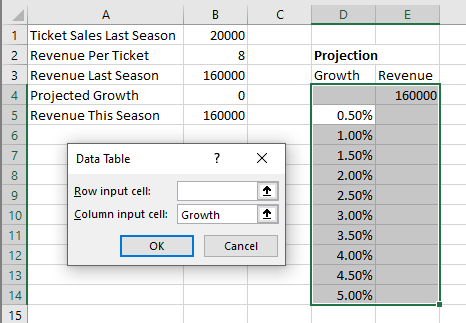
\includegraphics[width=\maxwidth{.95\linewidth}]{gfx/ch08_fig18}
	\caption{Setting Up the Data Table}
	\label{08:fig18}
\end{figure}

\begin{enumerate}[resume]	
	\item Click \fmtPopupButton{OK}.
\end{enumerate}

\begin{figure}[H]
	\centering
	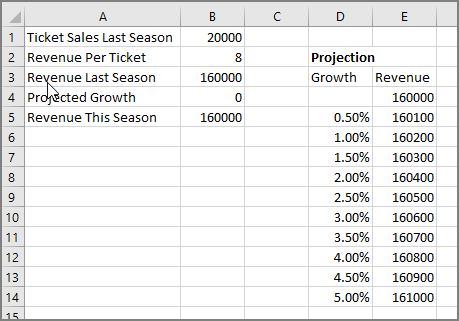
\includegraphics[width=\maxwidth{.95\linewidth}]{gfx/ch08_fig19}
	\caption{One-Variable Data Table}
	\label{08:fig19}
\end{figure}

The data table displays the projected revenue for each of the growth rates in column D. This analysis assumes that the number of tickets sold will increase. However, it is possible that ticket sales will decrease. Change the values in cells \fmtCellLocation{D5:D14} so some are negative and notice that the projected revenue automatically updates to display losses.

\begin{figure}[H]
	\centering
	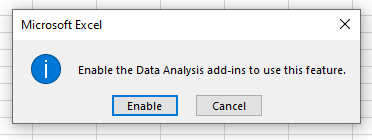
\includegraphics[width=\maxwidth{.95\linewidth}]{gfx/ch08_fig20}
	\caption{One-Variable Data Table With Negative Values}
	\label{08:fig20}
\end{figure}

\subsubsection{Two-Variable Data Table}

A mortgage is one of the most common loans. A mortgage for a home is a huge investment and borrowers must think carefully about the size of the monthly payment compared to their disposable income. A two-variable data table is very helpful in this type of decision.

Mortgages are commonly written for $ 10 $ to $ 30 $ year terms and the interest rate can vary widely, depending on many factors. For this example, assume the interest rate is between $ 5\% $ and $ 8.5\% $.

\begin{enumerate}
	\item Open a new worksheet.
	\item Name the worksheet \fmtWorksheetName{Mortgage}.
	\item Enter the following labels.
	
	\begin{itemize}
		\item In cell \fmtCellLocation{A1} enter \fmtTyping{Loan Amount}.
		\item In cell \fmtCellLocation{A2} enter \fmtTyping{Term in Years}.
		\item In cell \fmtCellLocation{A3} enter \fmtTyping{Interest Rate}.
		\item In cell \fmtCellLocation{A4} enter \fmtTyping{Payment}.
	\end{itemize}

	\item Adjust the width of column A so the labels fit in the column.
	\item To start the data table, enter these values in column B.
	
	\begin{itemize}
		\item In cell \fmtCellLocation{B1} enter \fmtTyping{100000}. This is the amount being borrowed.
		\item In cell \fmtCellLocation{B2} enter \fmtTyping{10}. This is the number of years to pay off the loan.
		\item In cell \fmtCellLocation{B3} enter \fmtTyping{0.05}. This is the interest rate being charged for the loan. \textit{Note}: the data table may be easier to read if cell \fmtCellLocation{B3} is formatted as \textit{percent} rather than \textit{general}. If the format is changed, be certain that it reads $ 5\% $.
		\item In cell \fmtCellLocation{B4}, enter \fmtTyping{=PMT(B3/12,B2*12,B1)}
	\end{itemize}

	\item Next, set up the data table area.
	\item In cell \fmtCellLocation{D4}, enter \fmtTyping{=B4}. This will ``seed'' the \fmtPopupButton{PMT} formula into the data table.
	\item In cells \fmtCellLocation{D5:D12}, enter \fmtTyping{0.05}, \fmtTyping{0.055}, \fmtTyping{0.06}, \fmtTyping{0.065}, \fmtTyping{0.07}, \fmtTyping{0.075}, \fmtTyping{0.08}, and \fmtTyping{0.085}.
	\item Format \fmtCellLocation{D5:D12} as percents.
	\item In cells \fmtCellLocation{E4:I4}, enter \fmtTyping{10}, \fmtTyping{15}, \fmtTyping{20}, \fmtTyping{25}, and \fmtTyping{30}.
	\item Highlight cells \fmtCellLocation{D4:I12} to contain the data table.
	\item Click \fmtRibbonButton{Data $ \Rightarrow $ Forecast $ \Rightarrow $ Data Table $ \Rightarrow $ What-If Analysis}.
	\item In the \fmtPopupBox{Row input cell} box, enter the reference for the data found in row 4. In the example, row 4 contains the loan term, and that is found in cell \fmtCellLocation{\$B\$2}. Note: this must be an absolute reference (with the dollar signs) or the data table function will fail.
	\item In the \fmtPopupBox{Column input cell} box, enter the reference for the data found in column D. In the example, column D contains the interest rate, and that is found in cell \fmtCellLocation{\$B\$3}. Note: this must be an absolute reference (with the dollar signs) or the data table function will fail.
	\item Click \fmtPopupButton{OK}.
\end{enumerate}

\begin{figure}[H]
	\centering
	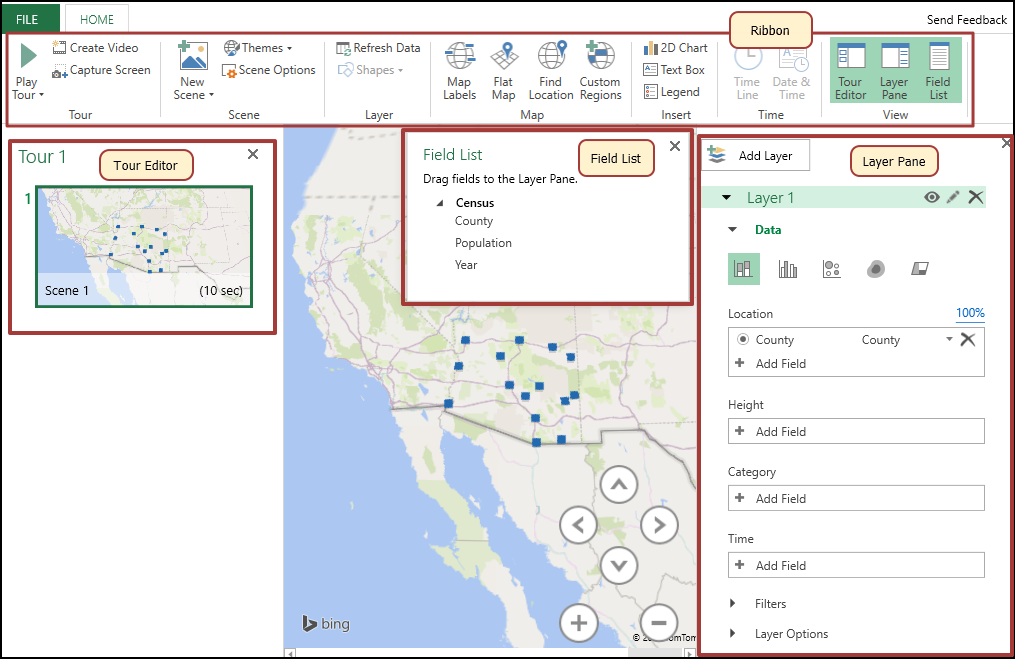
\includegraphics[width=\maxwidth{.95\linewidth}]{gfx/ch08_fig21}
	\caption{Setting Up The Two-Variable Data Table}
	\label{08:fig21}
\end{figure}

The data table displays the payment due for each combination of interest rate and loan term. Borrowers could then use this information to negotiate a rate and term that fits their budget. \textit{Note}: the payments are negative since they represent money leaving the borrower's bank account.

\begin{figure}[H]
	\centering
	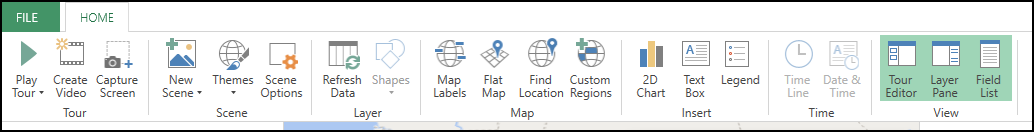
\includegraphics[width=\maxwidth{.95\linewidth}]{gfx/ch08_fig22}
	\caption{Completed Two-Variable Data Table}
	\label{08:fig22}
\end{figure}

\subsection{Scenarios}

Users may have data in a worksheet and want to change some of the variables to see the effect. For example, a business owner may want to consider ``best case'' and ``worst case'' values and then compare the results. This type of analysis is called a scenario in Excel.

\begin{enumerate}
	\item Open workbook \fmtWorkbookName{CH8-Scenario}.
\end{enumerate}

This workbook is a simple household budget for the Williams family. There are two working adults, Morgan and Phoenix. They are planning for several potential changes in their budget, including taking a ``once-in-a-lifetime'' vacation, starting college classes, and purchasing a new home. To help them decide on their best course of action, they are going to develop scenarios.

\begin{enumerate}[resume]
	\item Click \fmtRibbonButton{Data $ \Rightarrow $ Forecast $ \Rightarrow $ Scenario Manager $ \Rightarrow $ What-If Analysis}.
	\item Click \fmtPopupButton{Add} in the \fmtPopupBox{Scenario Manager} box.
\end{enumerate}

\begin{figure}[H]
	\centering
	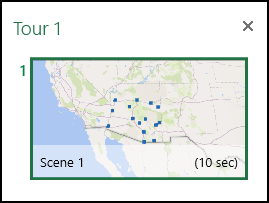
\includegraphics[width=\maxwidth{.95\linewidth}]{gfx/ch08_fig23}
	\caption{The Scenario Manager Dialog}
	\label{08:fig23}
\end{figure}

\begin{enumerate}[resume]	
	
	\item Enter these values in the \fmtPopupBox{Add Scenario} box.
	
	\begin{itemize}
		\item \textbf{Scenario name}: \fmtTyping{Current}. The first scenario will be the current budget and will work as a baseline for the other scenarios.
		\item \textbf{Changing Cells}: \fmtTyping{\$B\$4,\$B\$5,\$B\$9:\$B\$20}. These are the cells that the user can change for each scenario.
		\item \textbf{Comment}: \fmtTyping{Baseline Budget}. This is a brief description of the purpose for this scenario.
		\item \textbf{Prevent Changes}: Checked. This prevents the user from making changes to the Changing Cells other than with the scenario manager.
		\item \textbf{Hide}: Unchecked. This hides all of the changing cells.
	\end{itemize}

\end{enumerate}

\begin{figure}[H]
	\centering
	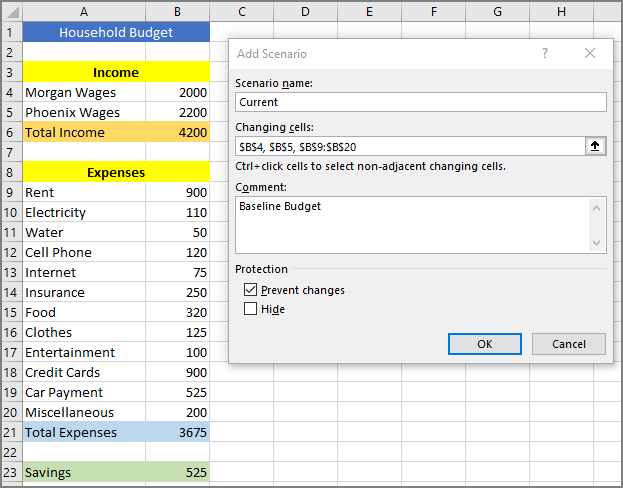
\includegraphics[width=\maxwidth{.95\linewidth}]{gfx/ch08_fig24}
	\caption{Adding A New Scenario}
	\label{08:fig24}
\end{figure}

\begin{enumerate}[resume]

	\item Click \fmtPopupButton{OK}.
	\item The \fmtPopupBox{Scenario Values} box will pop up. This is where the user can insert various values for the changeable cells. For this first scenario, none of the values will be changed, so click \fmtPopupButton{OK}.
	
\end{enumerate}

\begin{figure}[H]
	\centering
	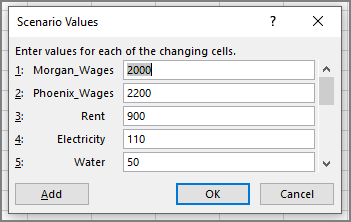
\includegraphics[width=\maxwidth{.95\linewidth}]{gfx/ch08_fig25}
	\caption{Changing Scenario Values}
	\label{08:fig25}
\end{figure}

\begin{enumerate}[resume]	
	
	\item The \fmtPopupBox{Scenario Manager} will pop up. It now indicates that there is one scenario named \textit{Current}. This scenario can be deleted or edited if desired, but click \fmtPopupButton{Add} to create a new scenario.
	
\end{enumerate}

\begin{figure}[H]
	\centering
	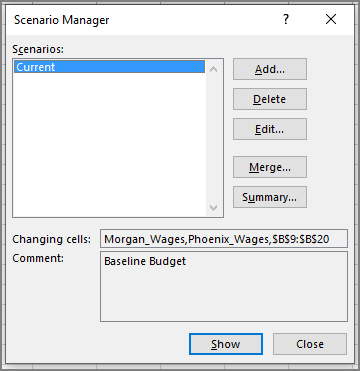
\includegraphics[width=\maxwidth{.95\linewidth}]{gfx/ch08_fig26}
	\caption{Scenario Manager With One Scenario}
	\label{08:fig26}
\end{figure}

\begin{enumerate}[resume]	
	
	\item Enter \fmtTyping{Vacation} for the scenario name, accept the default changing cells, and enter \fmtTyping{Budget for our vacation} as a comment. \fmtPopupBox{Leave Prevent} changes checked and \fmtPopupBox{Hide} unchecked.
	\item Click \fmtPopupButton{OK}.
	
\end{enumerate}

\begin{figure}[H]
	\centering
	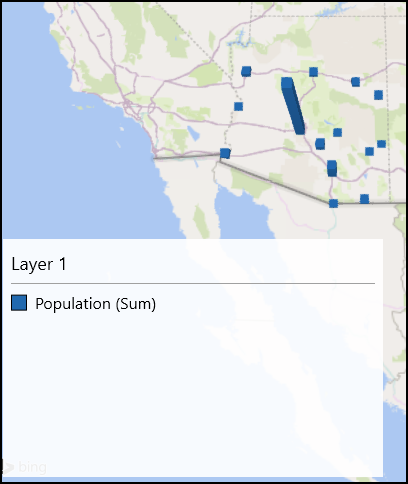
\includegraphics[width=\maxwidth{.95\linewidth}]{gfx/ch08_fig27}
	\caption{The Vacation Scenario}
	\label{08:fig27}
\end{figure}

\begin{enumerate}[resume]	
	
	\item Morgan and Phoenix believe that they need to increase their monthly savings significantly for their vacation. They decide to cut their food budget to $ 250 $, clothes to $ 50 $, entertainment to $ 50 $, and miscellaneous to $ 50 $. Enter those amounts in the \fmtPopupBox{Scenario Values} box.
	
\end{enumerate}

\begin{figure}[H]
	\centering
	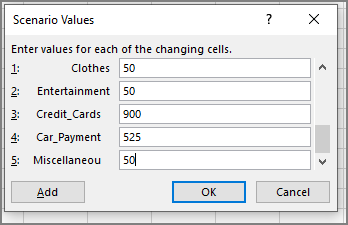
\includegraphics[width=\maxwidth{.95\linewidth}]{gfx/ch08_fig28}
	\caption{Vacation Scenario Values}
	\label{08:fig28}
\end{figure}

\begin{enumerate}[resume]	
	
	\item Click \fmtPopupButton{OK}.
	\item To see the result of the Vacation budget, select \fmtPopupBox{Vacation} and click \fmtPopupButton{Show} on the \fmtPopupBox{Scenario Manager} box.
	
\end{enumerate}

\begin{figure}[H]
	\centering
	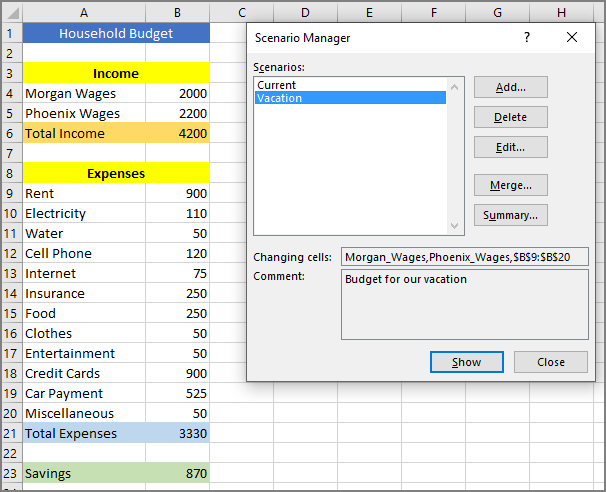
\includegraphics[width=\maxwidth{.95\linewidth}]{gfx/ch08_fig29}
	\caption{Vacation Scenario Results}
	\label{08:fig29}
\end{figure}

\begin{enumerate}[resume]	
	
	\item Morgan and Phoenix can now jump between the \fmtPopupBox{Current} and \fmtPopupBox{Vacation} budgets by selecting them in the \fmtPopupBox{Scenario Manager} box and clicking the \fmtPopupButton{Show} button.
	\item To reset the budget back to its baseline, select \fmtPopupBox{Current} and click \fmtPopupButton{Show} in the \fmtPopupBox{Scenario Manager} box.
	\item Next, they want to consider a budget for if one of them starts college. For that, they believe that they will have to find a smaller apartment near the campus and cut their other expenses significantly.
	\item Click \fmtPopupButton{Add} in the \fmtPopupBox{Scenario Manager}.
	\item Name the new scenario \fmtTyping{College} and enter \fmtTyping{Starting college classes} as a description. Accept all other default values for this scenario.
	\item In the Scenario Values box, enter $ 700 $ for rent, $ 100 $ for electricity, $ 200 $ for insurance, $ 175 $ for food, $ 50 $ for clothes, $ 50 $ for entertainment, and $ 50 $ for miscellaneous.
	\item To reset the budget back to its baseline, select \fmtPopupBox{Current} and click \fmtPopupButton{Show} in the \fmtPopupBox{Scenario Manager} box.
	\item Finally, Morgan and Phoenix want to consider purchasing a new house. Click \fmtPopupButton{Add} in the \fmtPopupBox{Scenario Manager} box to create a new scenario.
	\item Name the new scenario \fmtTyping{House} and enter \fmtTyping{Possible new house} as a description. Accept all other default values for this scenario.
	\item Even though they will not have rent, they will have a mortgage payment. For this worksheet, enter 1250 as rent to cover the cost of a mortgage payment. Enter 150 for electricty, 75 for water, 350 for insurance, 250 for food, 75 for clothes, 50 for entertainment, and 100 for miscellaneous.
	\item At this point, there are four scenarios and each can be viewed by clicking its name and \fmtPopupButton{Show} in the \fmtPopupBox{Scenario Manager} box. 
	
\end{enumerate}

\begin{figure}[H]
	\centering
	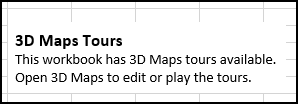
\includegraphics[width=\maxwidth{.95\linewidth}]{gfx/ch08_fig30}
	\caption{The Completed Scenario Manager}
	\label{08:fig30}
\end{figure}

\begin{enumerate}[resume]	
	
	\item It is possible to see a summary of all four scenarios in a single report. Click \fmtPopupButton{Summary} in the \fmtPopupBox{Scenario Manager} box.
	\item Excel offers to create a summary worksheet or a pivot table. For this exercise, select the \fmtPopupButton{Scenario summary} radio button, which will create a report.
	
\end{enumerate}

\begin{figure}[H]
	\centering
	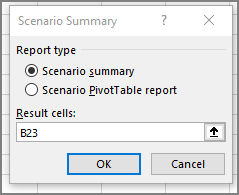
\includegraphics[width=\maxwidth{.95\linewidth}]{gfx/ch08_fig31}
	\caption{Scenario Summary Options}
	\label{08:fig31}
\end{figure}

\begin{enumerate}[resume]	
	
	\item The result cell, \fmtCellLocation{B23}, is the \textit{Savings} cell and this is the best option for reporting the results of each scenario.
	\item Click \fmtPopupButton{OK}.
	\item Excel produces a nice report that shows the values that were changed for each scenario and the result on their savings. 
\end{enumerate}

\begin{figure}[H]
	\centering
	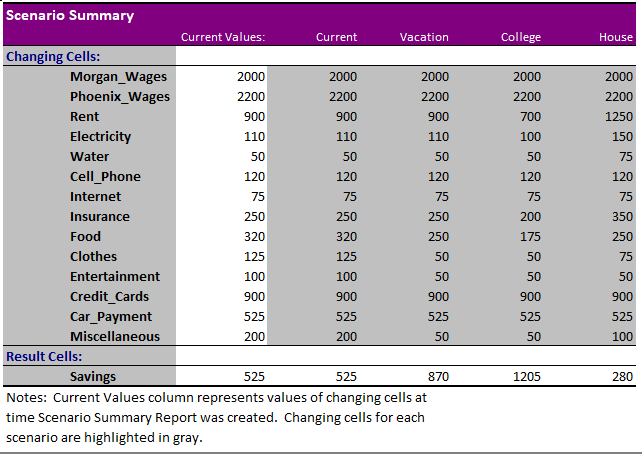
\includegraphics[width=\maxwidth{.95\linewidth}]{gfx/ch08_fig32}
	\caption{Scenario Summary Report}
	\label{08:fig32}
\end{figure}

\subsection{Goal Seeking}

Sometimes it is desirable to calculate a specific output for a formula by changing one of the input variables and this process is called ``Goal Seeking'' in Excel. As a demonstration of Goal Seeking, imagine that a mortgage of $ \$100000 $ is being negotiated and the buyer wants to keep payments under $ \$900 $ per month. If the mortgage will run $ 180 $ months ($ 15 $ years), what interest rate will lead to the maximum monthly payment possible under $ \$900 $?

\begin{enumerate}
	\item Open a new worksheet.
	\item Name the worksheet \fmtWorksheetName{Mortgage}
	\item Enter these labels in the first column.

	\begin{itemize}
		\item In cell \fmtCellLocation{A1} enter \fmtTyping{Loan Amount}.
		\item In cell \fmtCellLocation{A2} enter \fmtTyping{Term in Months}.
		\item In cell \fmtCellLocation{A3} enter \fmtTyping{Interest Rate}.
		\item In cell \fmtCellLocation{A4} enter \fmtTyping{Payment}.
	\end{itemize}

	\item Adjust the width of column A so the labels fit in the column.
	\item Enter the known values.

\begin{itemize}
	\item In cell \fmtCellLocation{B1} enter \fmtTyping{100000}. This is the amount being borrowed.
	\item In cell \fmtCellLocation{B2} enter \fmtTyping{180}. This is the number of months to pay off the loan. 
\end{itemize}
\end{enumerate}

\begin{center}
	\begin{infobox}{Note}
		Although the desired payment amount is known, do not enter it as a value because it will be calculated by a formula. Instead, enter the formula and then specify the desired payment later.
	\end{infobox}
\end{center}

\begin{enumerate}[resume]
	\item Enter a formula to calculate the payment. In cell \fmtCellLocation{B4}, type \fmtTyping{=PMT(B3/12,B2,B1)} to calculate the payment amount.
	\item The formula refers to cells \fmtCellLocation{B1} and \fmtCellLocation{B2}, which contain values specified earlier. The formula also refers to cell \fmtCellLocation{B3}, which is where \textit{Goal Seek} will enter the interest rate. The formula divides the value in \fmtCellLocation{B3} by $ 12 $ because a monthly payment is specified and the \fmtPopupButton{PMT} function assumes an annual interest rate.
	\item Because there is no value in cell \fmtCellLocation{B3}, Excel assumes a $ 0 $\% interest rate and returns a payment of \$$ 555.56 $. That value can be ignored for now.
\end{enumerate}

Use \textit{Goal Seek} to determine the optimum interest rate for the payment desired.

\begin{enumerate}
	\item Click \fmtRibbonButton{Data $ \Rightarrow $ Forecast $ \Rightarrow $ Goal Seek $ \Rightarrow $ What-If Analysis}.
	\item In the \fmtPopupBox{Set cell} box, enter the reference for the cell that contains the formula to be resolved. In the example, this formula is in cell \fmtCellLocation{B4}.
	\item In the \fmtPopupBox{To value} box, enter the desired formula result \fmtTyping{-900} in this example. \textit{Note} this number is negative because it represents money being paid out of a checking account.
	\item In the \fmtPopupBox{By changing cell} box, enter the reference for the cell that contains the value to adjust, or \fmtCellLocation{B3} in this example. \textit{Note}: The cell that Goal Seek changes must be referenced by the formula in the cell specified in the \fmtPopupBox{Set cell} box.
	
\end{enumerate}

\begin{figure}[H]
	\centering
	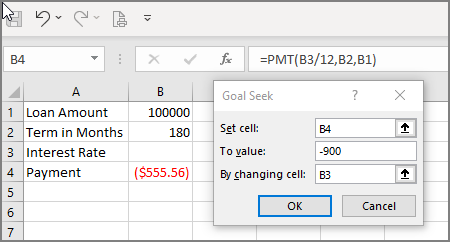
\includegraphics[width=\maxwidth{.95\linewidth}]{gfx/ch08_fig33}
	\caption{Setting Up Goal Seeking}
	\label{08:fig33}
\end{figure}

\begin{enumerate}[resume]	
	\item Click \fmtPopupButton{OK}.
\end{enumerate}

Excel calculates an interest rate of $ 0.07021 $ ($ 7\% $) to yield a monthly payment of $ \$900 $. To save that amount in the worksheet, click \fmtPopupButton{OK} but to cancel this process and return to the original worksheet values, click \fmtPopupButton{Cancel}.

\begin{figure}[H]
	\centering
	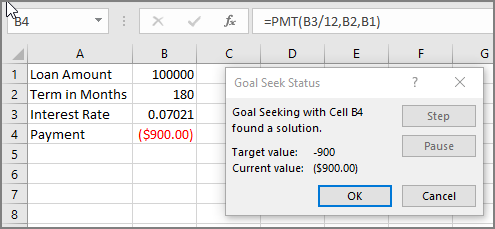
\includegraphics[width=\maxwidth{.95\linewidth}]{gfx/ch08_fig34}
	\caption{Results of Goal Seeking}
	\label{08:fig34}
\end{figure}

\subsection{Solver}

The Excel Solver is used to find an optimum solution for complex business problems. As an example, Solver would evaluate multiple parameters to find the best mix of products for a company to manufacture. For this exercise, the \textit{PeopleMover Transportation} company wants to create a spreadsheet that will help their planners determine the best mix of motor coaches for a contract.

\begin{enumerate}
	\item Open workbook \fmtWorkbookName{CH8-Solver}.
\end{enumerate}

This workbook has only one worksheet, \fmtWorksheetName{Planner}. The worksheet has some information already filled in. The company has four different coaches: \textit{Deluxe}, \textit{Large}, \textit{Mid-Size}, and \textit{Mini}. For each type of coach, the passenger capacity is listed. Also, the cost of operating the coach per mile is specified. Finally, the number that the company has on hand is listed. For example, a \textit{Deluxe} coach can carry $ 56 $ passengers at a cost of \$$ 2.80 $ per mile to operate. The company has two \textit{Deluxe} coaches on hand.

Cells \fmtCellLocation{A14:B15} on the worksheet is where information about a trip is entered. For example, the worksheet is set up for a trip of $ 300 $ miles that $ 350 $ people want to take.

The goal is to have Excel calculate the optimum mix of coaches to get a total capacity (cell \fmtCellLocation{B11}) greater than the number of riders (\fmtCellLocation{B15}) at a minimum cost (cell \fmtCellLocation{B12}). This is a perfect job for Solver.

Solver is part of Excel, but it is considered an Add-in and must be activated before it can be used.

\begin{enumerate}[resume]
	\item Click \fmtRibbonTab{File} to open the backstage view.
	\item In the backstage view, click \fmtRibbonButton{Options} at the bottom of the left-hand menu.
	
\end{enumerate}

\begin{figure}[H]
\centering
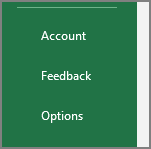
\includegraphics[width=\maxwidth{.95\linewidth}]{gfx/ch08_fig35}
\caption{The Options Button in the Backstage View}
\label{08:fig35}
\end{figure}

\begin{enumerate}[resume]	
	
	\item Click \fmtPopupButton{Add-ins} in the left-hand menu of the \fmtPopupBox{Excel Options} pop-up box.
	\item Select \fmtPopupBox{Excel Add-ins} in the drop-down menu at the bottom of the \fmtPopupBox{Add-ins} tab.
	\item Click \fmtPopupButton{Go}.
	
\end{enumerate}

\begin{figure}[H]
\centering
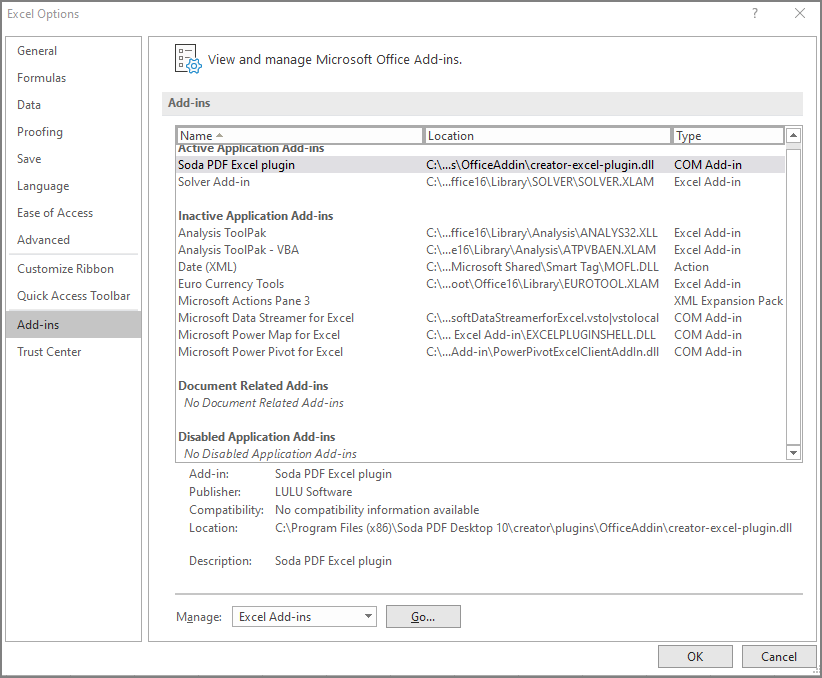
\includegraphics[width=\maxwidth{.95\linewidth}]{gfx/ch08_fig36}
\caption{The Add-ins Manager}
\label{08:fig36}
\end{figure}

\begin{enumerate}[resume]	
	
	\item Click the checkbox beside \fmtPopupBox{Solver Add-in} in the \fmtPopupBox{Add-ins} pop-up box.
	
\end{enumerate}

\begin{figure}[H]
	\centering
	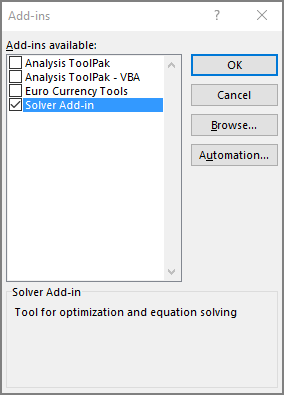
\includegraphics[width=\maxwidth{.95\linewidth}]{gfx/ch08_fig37}
	\caption{Activating The Solver Add-In}
	\label{08:fig37}
\end{figure}

\begin{enumerate}[resume]	
	\item Click \fmtPopupButton{OK}.
\end{enumerate}

Notice that there is a new \fmtRibbonButton{Solver} button at \fmtRibbonButton{Data $ \Rightarrow $ Analyze}.

\begin{enumerate}[resume]
	\item To set up the solver, click \fmtRibbonButton{Data $ \Rightarrow $ Analyze $ \Rightarrow $ Solver}.
	\item In the \fmtPopupBox{Set Objective} box, click the selector button and then click cell \fmtCellLocation{B12} to select it. This sets the Solver to solve for the total cost of the coaches. (Note: since cell \fmtCellLocation{B12} has a name, the Solver displays the name \textit{Ttl\_Cost} instead of \fmtCellLocation{B12}.)
	\item For \fmtPopupBox{To}, Select the \fmtPopupButton{Min} radio button. This sets the Solver to look for the minimum cost for the mix of coaches it recommends.
	\item Click \fmtPopupButton{Add} beside the \fmtPopupBox{Subject to the Constraints} box to add the constraints for the Solver.
	\item Add two new constraints for cell \fmtCellLocation{E6}. First, specify that it must be $ <= $ cell \fmtCellLocation{D6}. That means that the number of Deluxe coaches allotted for the trip must be less than or equal to the number on hand. Second, specify that cell \fmtCellLocation{E6} must contain an integer since it is not possible to allot a partial coach.
	\item Add constraints for Large, Mid-Size, and Mini coaches that are similar to those for the Deluxe coach.
	\item Add a constraint that \fmtCellLocation{B11} must be $ >= $ \fmtCellLocation{B15} since all riders need to have a seat on a coach.
	\item Check the box for ``Make Unconstrained Variables Non-Negative'' since it is not possible to have a negative number of coaches or riders.
	 \item For \fmtPopupBox{Select a Solving Method}, the default is \fmtPopupButton{GRG Nonlinear}. This is normally a good option to use.
	 
\end{enumerate}

\begin{figure}[H]
	\centering
	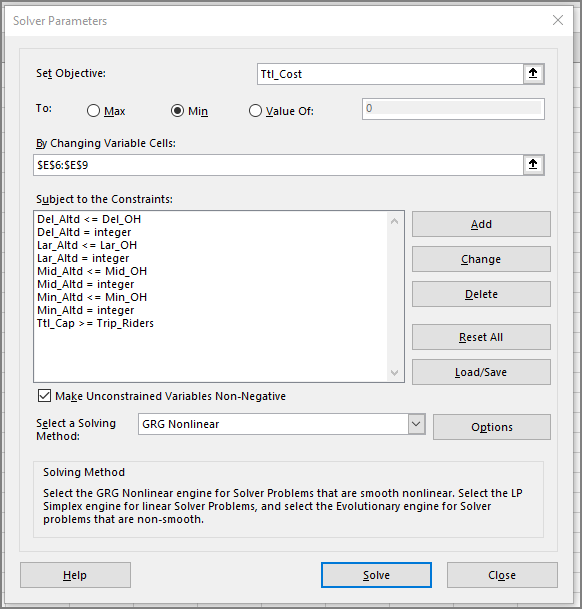
\includegraphics[width=\maxwidth{.95\linewidth}]{gfx/ch08_fig38}
	\caption{The Solver Parameters}
	\label{08:fig38}
\end{figure}

\begin{enumerate}[resume]	 
	 \item Click \fmtPopupButton{Solve}.
\end{enumerate}

After a few seconds, the Solver will calculate the mix of coaches that yields the least cost. Notice that the Solver changed the Allotted values for each of the coaches along with the Total Capacity and Total Cost to match the optimal solution. Also, notice that the total coach capacity is $ 354 $ for the solution while there are only $ 350 $ riders, so there will be four empty seats on the coaches. This solution will cost PeopleMover Transportation \$$ 4,575.00 $ so they would have to price tickets appropriately.

\begin{figure}[H]
	\centering
	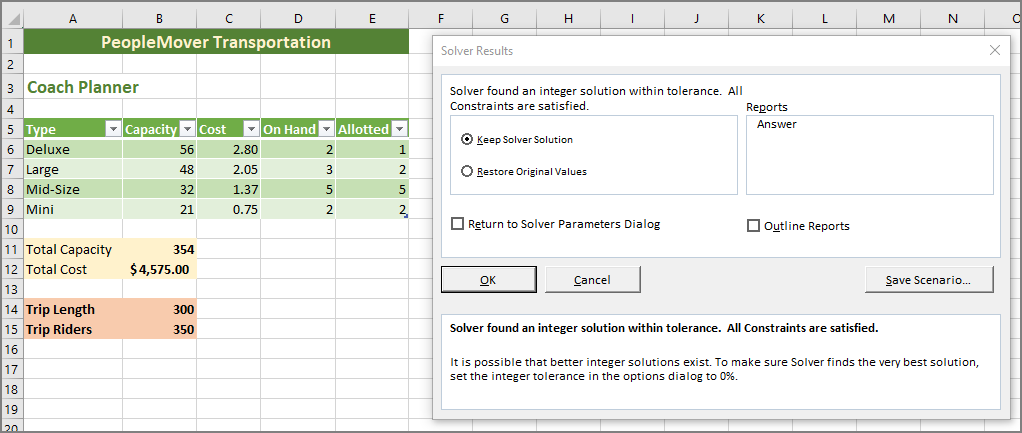
\includegraphics[width=\maxwidth{.95\linewidth}]{gfx/ch08_fig39}
	\caption{Solver Results}
	\label{08:fig39}
\end{figure}

To save this solution, click \fmtPopupBox{Keep Solver Solution} and \fmtPopupButton{OK}. To return to the original values, click \fmtPopupBox{Restore Original Values} and \fmtPopupButton{OK}. Finally, this solution can be saved as a scenario so it can be compared with other solutions.

\begin{center}
	\begin{tkwbox}{Key Take-Aways}
		\textbf{What-If Analysis}
		\\
		\begin{itemize}
			\setlength{\itemsep}{0pt}
			\setlength{\parskip}{0pt}
			\setlength{\parsep}{0pt}
			
			\item Data tables are built by processing numeric inputs using Excel functions and formulas.
			\item Scenarios create various sets of inputs to compare the resulting output.
			\item Goal seeking finds an optimum input to achieve a specific goal.
			\item The Solver finds optimal solutions to complex business problems.
			
		\end{itemize}
	\end{tkwbox}
\end{center}

\section{Chapter Practice}

\subsection{Voting Map}

\begin{enumerate}
	\item Open workbook \fmtWorkbookName{PR8-Data}.
\end{enumerate}

This workbook includes the percent of Arizona voters who voted for Trump, Clinton, and Other by county in the $ 2016 $ Presidential Election. Mapping this data will help reveal information about the areas of the state the support each of the parties.

\begin{enumerate}[resume]
	\item Click cell \fmtCellLocation{A3:C18} to activate that range of cells.
	\item Click \fmtRibbonButton{Insert $ \Rightarrow $ Charts $ \Rightarrow $ Maps}.
	\item Select \fmtRibbonButton{Filled Map}.
	\item Click the map icon.
	\item Once the map is created, change the title to ``Trump Support''.
	\item Double-click the map area, then select the \fmtPopupBox{Data Series} tab (it looks like columns). In the \fmtPopupBox{Series Color} section, select \textit{Red} for the Maximum value and \textit{Orange Accent 2} (a pale orange) for the Minimum value. 
\end{enumerate}

\begin{figure}[H]
	\centering
	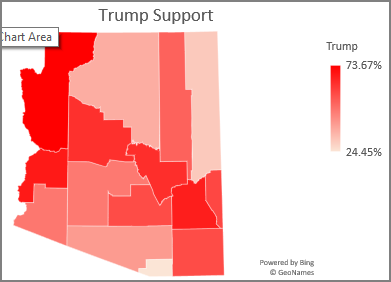
\includegraphics[width=\maxwidth{.95\linewidth}]{gfx/ch08_fig40}
	\caption{The Trump Support Map}
	\label{08:fig40}
\end{figure}

Excel creates a map of Arizona where Trump's percentage is indicated by a red color. The greater his percentage the brighter the color. For example, Mohave County in the top left corner (the northwest part of the state) is bright red because 73.67\% of the voters there supported Trump.

\begin{enumerate}[resume]
	\item Click off of the \textit{Trump Support} map and move it to the top right corner of the worksheet.
	\item Click cell \fmtCellLocation{A3:B18} and then holding down the \fmtKeystroke{Control} key, click \fmtCellLocation{D3:D18} to activate those cells.
	\item Click \fmtRibbonButton{Insert $ \Rightarrow $ Charts $ \Rightarrow $ Maps}.
	\item Select \fmtRibbonButton{Filled Map}.
	\item Click the map icon.
	\item Once the map is created, change the title to ``Clinton Support''.
	\item The default blue color is appropriate for Clinton's map, so that does not need to be changed.
\end{enumerate}

\begin{figure}[H]
	\centering
	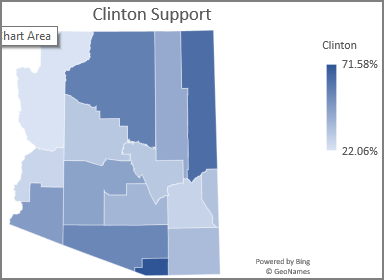
\includegraphics[width=\maxwidth{.95\linewidth}]{gfx/ch08_fig41}
	\caption{The Clinton Support Map}
	\label{08:fig41}
\end{figure}

\begin{enumerate}[resume]
	\item Click off of the \textit{Clinton Support} map and move it to the bottom right corner of the worksheet.
	\item Create a new colum beween D and E.
	\item Enter \fmtTyping{Delta} in \fmtCellLocation{E3}.
	\item Click cell \fmtCellLocation{A3:B18} and then holding down the \fmtKeystroke{Control} key, click \fmtCellLocation{E3:E18} to activate those cells.
	\item Click \fmtRibbonButton{Insert $ \Rightarrow $ Charts $ \Rightarrow $ Maps}.
	\item Select \fmtRibbonButton{Filled Map}.
	\item Click the map icon.
	\item Once the map is created, change the title to ``Party Strength''.
	\item Double-click the map area to open the \fmtPopupBox{Format Chart Area} panel.
	\item Click anywhere on the map to open the \fmtPopupBox{Format Data Series} panel.
	\item Open the \fmtPopupBox{Series} tab by clicking the \fmtPopupButton{Columns} icon.
	
\end{enumerate}

\begin{figure}[H]
	\centering
	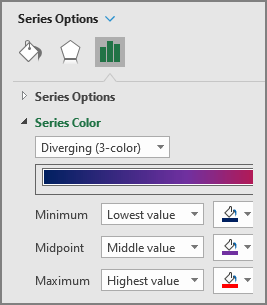
\includegraphics[width=\maxwidth{.95\linewidth}]{gfx/ch08_fig42}
	\caption{Setting The Color Options}
	\label{08:fig42}
\end{figure}

\begin{enumerate}[resume]	
	\item In the \fmtPopupBox{Series Color} section, select \fmtPopupButton{Diverging (3-color)}.
	\item Select blue for the Lowest Value, purple for the Middle Value, and red for the Highest value.
\end{enumerate}

\begin{figure}[H]
	\centering
	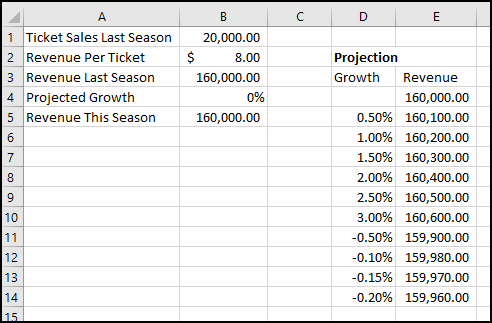
\includegraphics[width=\maxwidth{.95\linewidth}]{gfx/ch08_fig43}
	\caption{The Party Strength Map}
	\label{08:fig43}
\end{figure}

The last map shows the Republican counties in red, the Democratic counties in blue, and the swing counties in purple and indicates the relative strength of each party by county.

\section{Scored Assessment}

\subsection{Product Mix}

The \textit{Giant Electronics} company is a local small business that sells discounted electronic devices, like televisions and computers. The owners, Addison and Kelsey, are planning for their annual spring promotion and want to create a good mix of sale items.

\begin{enumerate}
	\item Open workbook \fmtWorkbookName{SC8-Data}.
\end{enumerate}

This workbook has only one worksheet, \fmtWorksheetName{Planner}. The worksheet already has the solver set up and has some information filled in. Addison and Kelsey are planning to promote four items, a television, a computer, various game cartridges, and a camera. The worksheet shows the cost for each item; for example, each television set costs them \$$ 899 $. The price they intend to sell each item is also noted. For example, televisions will sell for \$$ 1049 $. The profit for each item is calculated by subtracting the cost from the price. Finally, the \textit{To Order} column lists how many of each item they should order for their sale.

In cell \fmtCellLocation{B11}, under the Planner table, Addison and Kelsey indicate how much they want to invest in the sale. The worksheet initially indicates a \$$ 50,000 $ investment.

Cell \fmtCellLocation{B13} has a formula that calculates the total cost of whatever they decide to order and \fmtCellLocation{B14} has a formula that calculates the total profit for those items.

\begin{enumerate}
	\item Click \fmtRibbonButton{Data $ \Rightarrow $ Analyze $ \Rightarrow $ Solver}.
	\item In the \fmtPopupBox{Set Objective} box, click the selector button and then click cell \fmtCellLocation{B14} to select it. This sets the Solver to solve for the total profit of the sale items. (Note: since cell \fmtCellLocation{B14} has a name, the Solver displays the name \textit{Ttl\_Profit} instead of \fmtCellLocation{B14}.)
	\item For \fmtPopupBox{To}, Select the \fmtPopupButton{Max} radio button. This sets the Solver to look for the maximum profit for the mix of products it recommends.
	\item The constraints are already defined. These will be changed later, but the initial configuration requires the total cost to be less than the investment. The configuration also requires all orders to be integers (it is not possible to order a fraction of a television) and there are some constraints on the number of items that can be ordered.
	\item Make sure the \fmtPopupBox{GRG Nonlinear} is the solving method.
\end{enumerate}

\begin{figure}[H]
	\centering
	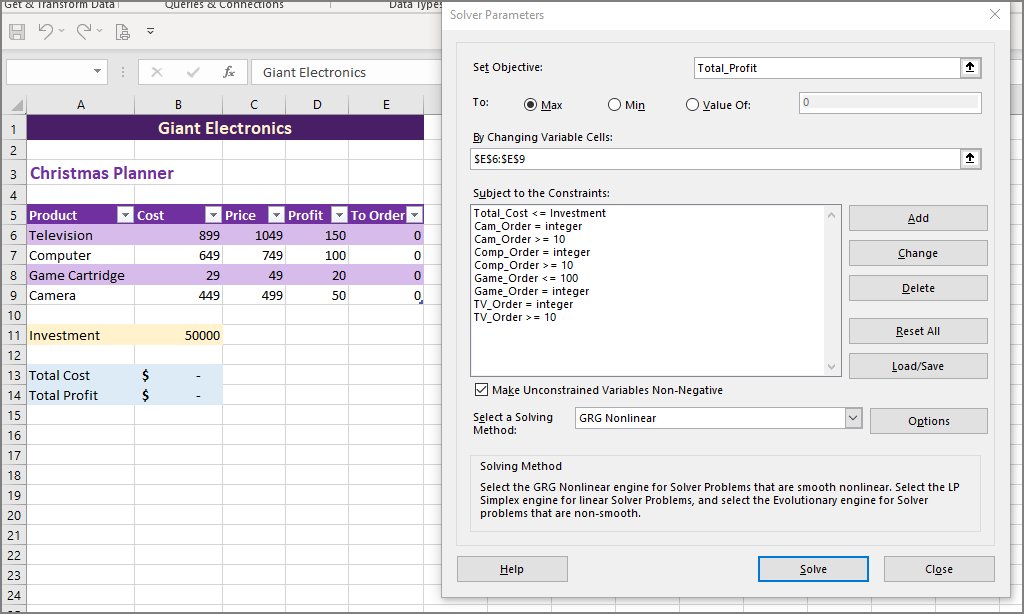
\includegraphics[width=\maxwidth{.95\linewidth}]{gfx/ch08_fig44}
	\caption{Solver Initial Setup}
	\label{08:fig44}
\end{figure}

\begin{enumerate}[resume]
	\item Click \fmtPopupButton{Solve}.
\end{enumerate}

\begin{figure}[H]
	\centering
	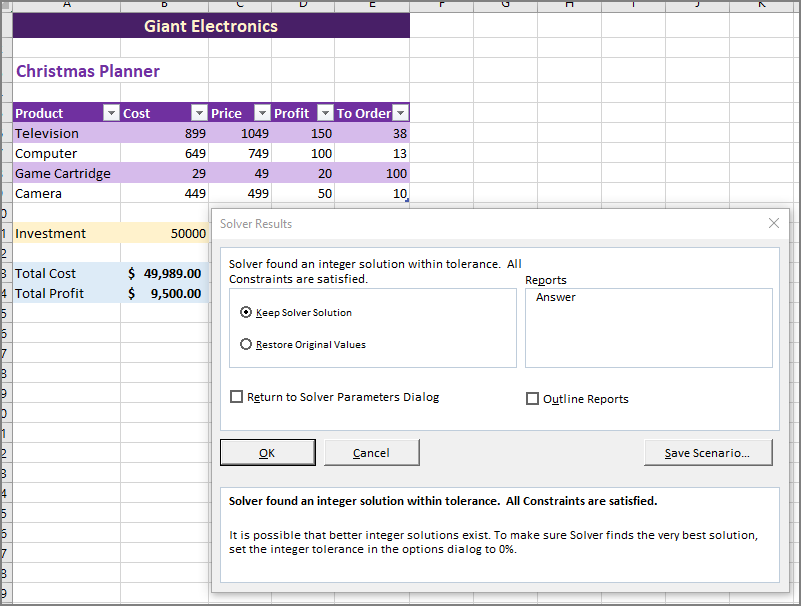
\includegraphics[width=\maxwidth{.95\linewidth}]{gfx/ch08_fig45}
	\caption{Solver Initial Solution}
	\label{08:fig45}
\end{figure}

Solver determined that the optimum mix of products was $ 38 $ televisions, $ 13 $ computers, $ 100 $ Game cartridges, and $ 10 $ cameras. This will cost Addison and Kelsey \$$ 49,989 $, just under their \$$ 50,000 $ limit and will net them a profit of \$$ 9,500 $. 

\begin{enumerate}[resume]
	\item Click \fmtPopupButton{Save Scenario}.
	\item Name the scenario \fmtTyping{Initial Attempt}.
	\item Click \fmtPopupBox{Restore Original Values} in the Results dialog box to return the Planner table to its original state.
	\item Click \fmtPopupBox{Answer} in the Reports dialog box. This makes Excel generate a report named \textit{Answer Report 1}.
	\item Click \fmtPopupButton{OK}.
	\item Excel creates a report on a new worksheet named \fmtWorksheetName{Answer Report 1}. This makes it easy to come back to this solution later.
	\item Click \fmtRibbonButton{Data $ \Rightarrow $ Forecast $ \Rightarrow $ What-If}.	Notice that Excel placed that first scenario, \textit{Initial Attempt}, in the scenario manager for later reference.
	\item Click \fmtPopupButton{Close} to close the scenario manager.
\end{enumerate}

Addison and Kelsey decide that they want to sell more than $ 10 $ cameras and they think that $ 100 $ game cartridges are too many. Adjust the parameters in the Solver and run it again.

\begin{enumerate}
	\item Click \fmtRibbonButton{Solver $ \Rightarrow $ Analyze $ \Rightarrow $ What-If}.
	\item Click \fmtPopupBox{Cam\_Order $ >=$ $ 10 $} to select it and then click \fmtPopupButton{Change}.
	\item Change the constraint to $ 20 $ and click \fmtPopupButton{OK}.
	\item Click \fmtPopupBox{Game\_Order $ <=$ $ 100 $} to select it and then click \fmtPopupButton{Change}.
	\item Change the constraint to $ 50 $ and click \fmtPopupButton{OK}.
	\item Click \fmtPopupButton{Solve}.
	\item Notice that Excel has now adjusted the order column so only $ 50 $ game cartridges and $ 20 $ cameras will be ordered. Also notice that the profit has dropped to \$$ 8,500 $. 
	\item Click \fmtPopupButton{Save Scenario} and name it \fmtTyping{20 Cameras}.
	\item Click \fmtPopupBox{Answer} in the Reports dialog box. This makes Excel generate a report named \textit{Answer Report 2}.
	\item Select \fmtPopupBox{Restore Original Values} and click \fmtPopupButton{OK}.
\end{enumerate}

Addison and Kelsey would like to boost their profit a bit so they decide to adjust the selling price for two items. They think the television could sell for \$ $ 1199 $ and the computer for \$$ 999 $. 

\begin{enumerate}
	\item Click \fmtCellLocation{C6} to activate that cell and enter $ 1199 $ for the new television selling price.
	\item Click \fmtCellLocation{C7} to activate that cell and enter $ 999 $ for the new computer selling price.
	\item Click \fmtRibbonButton{Solver $ \Rightarrow $ Analyze $ \Rightarrow $ What-If}.
	\item Click \fmtPopupButton{Solve} on the \fmtPopupBox{Solver Parameters} dialog box.
	\item Click \fmtPopupButton{Save Scenario} and name it \fmtTyping{Expensive Televisions}.
	\item Click \fmtPopupBox{Answer} in the Reports dialog box. This makes Excel generate a report named \textit{Answer Report 3}.
	\item Select \fmtPopupBox{Restore Original Values} and click \fmtPopupButton{OK}.
\end{enumerate}

The Solver decreased the number of televisions to $ 10 $ but increased the number of computers to $ 47 $. This change will create a profit of \$$ 21,450 $.

Addison and Kelsey could continue adjusting the sale prices and the maximum number of each item to order to come to what they believe is the optimum mix of products for their spring sale.





